% 
% Annual Cognitive Science Conference
% Sample LaTeX Paper -- Proceedings Format
% 

% Original : Ashwin Ram (ashwin@cc.gatech.edu)       04/01/1994
% Modified : Johanna Moore (jmoore@cs.pitt.edu)      03/17/1995
% Modified : David Noelle (noelle@ucsd.edu)          03/15/1996
% Modified : Pat Langley (langley@cs.stanford.edu)   01/26/1997
% Latex2e corrections by Ramin Charles Nakisa        01/28/1997 
% Modified : Tina Eliassi-Rad (eliassi@cs.wisc.edu)  01/31/1998
% Modified : Trisha Yannuzzi (trisha@ircs.upenn.edu) 12/28/1999 (in process)
% Modified : Mary Ellen Foster (M.E.Foster@ed.ac.uk) 12/11/2000
% Modified : Ken Forbus                              01/23/2004
% Modified : Eli M. Silk (esilk@pitt.edu)            05/24/2005
% Modified: Niels Taatgen (taatgen@cmu.edu) 10/24/2006

%% Change ``a4paper'' in the following line to ``letterpaper'' if you are
%% producing a letter-format document.

\documentclass[10pt,letterpaper]{article}

% uncomment below to put in cogsci format
%\usepackage{cogsci}

\usepackage{pslatex}
\usepackage{apacite}
\usepackage{amsmath}
\usepackage{graphicx}
\usepackage{color}
\usepackage{amssymb}

\usepackage{algorithmic}
\usepackage{algorithm}
\usepackage{amsthm}
\usepackage{float}
\usepackage{mathrsfs}
\usepackage{fullpage}


\newcommand{\footnoteremember}[2]{
\footnote{#2}
\newcounter{#1}
\setcounter{#1}{\value{footnote}}
}
\newcommand{\footnoterecall}[1]{
\footnotemark[\value{#1}]
}


%%%%%%%%%%%%%%%%%%%%%%%%%%%%%%%%%%%%%%%%%%%%%%%%%%%%%%%%%%%%%%%%%%%%%%
% title
%%%%%%%%%%%%%%%%%%%%%%%%%%%%%%%%%%%%%%%%%%%%%%%%%%%%%%%%%%%%%%%%%%%%%%
\title{{\bf VS265 Final Project}\\Exemplar storage in associative memory systems}
 
%%%%%%%%%%%%%%%%%%%%%%%%%%%%%%%%%%%%%%%%%%%%%%%%%%%%%%%%%%%%%%%%%%%%%%
% authors
%%%%%%%%%%%%%%%%%%%%%%%%%%%%%%%%%%%%%%%%%%%%%%%%%%%%%%%%%%%%%%%%%%%%%%
\author{{\large \bf Joshua T. Abbott (joshua.abbott@berkeley.edu)\footnoteremember{myfootnote}{The authors contributed equally to this work.}} \\
 {\large \bf Jessica B. Hamrick (jhamrick@berkeley.edu)\footnoterecall{myfootnote}} \\
% {\large \bf Thomas L. Griffiths (tom\_griffiths@berkeley.edu)} \\
  Department of Psychology, University of California, Berkeley, CA 94720 USA}

\date{}

\begin{document}

\maketitle

%%%%%%%%%%%%%%%%%%%%%%%%%%%%%%%%%%%%%%%%%%%%%%%%%%%%%%%%%%%%%%%%%%%%%%
% abstract
%%%%%%%%%%%%%%%%%%%%%%%%%%%%%%%%%%%%%%%%%%%%%%%%%%%%%%%%%%%%%%%%%%%%%%
\begin{abstract}
This is the abstract.

% \textbf{Keywords:} 
% Sparse Distributed Memory systems, Bayesian inference, Exemplar model, Rational Process Model, Importance Sampling.
\end{abstract}

%%%%%%%%%%%%%%%%%%%%%%%%%%%%%%%%%%%%%%%%%%%%%%%%%%%%%%%%%%%%%%%%%%%%%%
% introduction
%%%%%%%%%%%%%%%%%%%%%%%%%%%%%%%%%%%%%%%%%%%%%%%%%%%%%%%%%%%%%%%%%%%%%%
\section{Introduction}

% something broad about prob models of cognition 
\cite{griffiths2010probabilistic,tenenbaum2011grow}

% something about issues with prob models
\cite{kahneman1972subjective,gigerenzer2000simple}

% something about marrs levels and that approach
\cite{marr82,anderson90}

% something about addressing these issues with RPM and bridging levels
\cite{sanborn2010rational,griffiths2012bridging}

% in particular we look at exemplar model approx
\cite{Shi2010}

%%%%%%%%%%%%%%%%%%%%%%%%%%%%%%%%%%%%%%%%%%%%%%%%%%%%%%%%%%
% subsection - exemplar models / IS for Bayes 
%%%%%%%%%%%%%%%%%%%%%%%%%%%%%%%%%%%%%%%%%%%%%%%%%%%%%%%%%%
\subsection{Exemplar models and Bayesian inference}

% maybe start with a simple example of exemplar models like Lei does.. 

% what is an exemplar model
% In an \textit{exemplar model} model of memory, people store individual instances of observations in memory (as an \textit{exemplar}) and evaluate new observations by activating these stored exemplars as a function of their similarity to this novel event \cite{medin1978context,nosofsky1986attention}. More formally, let $X^{*} = \{ x^{*}_{1}, x^{*}_{2}, \ldots, x^{*}_{n} \}$ represent a set of $n$ stored exemplars, and define $s(x,x^{*})$ to be a similarity function measuring the distance between an observation $x$ and a stored exemplar $x^{*}$. 

% -- i dont know if i like the above, i'm too tired..

% something about an identification task

\begin{equation}
	p_{r}(x^{*}_{i}|x)=\frac{s(x,x^{*}_{i})}{\sum^{n}_{j=1}s(x,x^{*}_{j})}
\end{equation}

% something about exemp models can do prob. categorization
\cite{ashby1995categorization}

% however a more general form of exemp models is

\begin{equation}
	\hat{f}(x)=\frac{\sum^{n}_{j=1}f_{j}\,s(x,x^{*}_{j})}{\sum^{n}_{j=1}s(x,x^{*}_{j})}
\end{equation}

% very brief bayes

% very brief intro to importance sampling

\cite{neal1993probabilistic,Shi2010}

%%%%%%%%%%%%%%%%%%%%%%%%%%%%%%%%%%%%%%%%%%%%%%%%%%%%%%%%%%
% subsection - previous implementations: RBFs
%%%%%%%%%%%%%%%%%%%%%%%%%%%%%%%%%%%%%%%%%%%%%%%%%%%%%%%%%%
\subsection{Neural implementations of Importance Sampling}
\cite{Shi2009}

% review Lei's components of an importance sampler

% math of RBF

% *** interesting because the RBF network is not cognitively satisfying \\
% **** all grandmother cells (and the proposed spiking neuron model was using an RBF too..) \\
% **** not robust \\


% what is an associative memory model

% something about distributed memory

% the rest of the paper explores the role of exemplars and associative memory


%%%%%%%%%%%%%%%%%%%%%%%%%%%%%%%%%%%%%%%%%%%%%%%%%%%%%%%%%%%%%%%%%%%%%%
% associative models of memory
%%%%%%%%%%%%%%%%%%%%%%%%%%%%%%%%%%%%%%%%%%%%%%%%%%%%%%%%%%%%%%%%%%%%%%
\section{Associative models of memory}



% for a full discussion, check out
\cite{Keeler1988}

%%%%%%%%%%%%%%%%%%%%%%%%%%%%%%%%%%%%%%%%%%%%%%
% subsection - Hopfield networks
%%%%%%%%%%%%%%%%%%%%%%%%%%%%%%%%%%%%%%%%%%%%%%
\subsection{Hopfield networks}
\cite{Hopfield1982}

% hopfield nets are auto-associative, meaning the whole network converges to one particular pattern given an input and does not leave this state until presented with a new input. 

% simple math of hopnet (Hebbian learning rule)


% known issues:
% (1) storage capacity is small fraction of number of number of neurons
% (2) can't do temporal sequences
% (3) unrealistic model of brain - requires symmetric connections
% (4) bad with correlated patterns

%%%%%%%%%%%%%%%%%%%%%%%%%%%%%%%%%%%%%%%%%%%%%%
% subsection - SDM
%%%%%%%%%%%%%%%%%%%%%%%%%%%%%%%%%%%%%%%%%%%%%%
\subsection{Sparse distributed memory systems}
\cite{Kanerva1988,Kanerva1993}

% SDMs can be a whole range of foo-associative


%%%%%%%%%%%%%%%%%%%%%%%%%%%%%%%%%%%%%%%%%%%%%%%%%%%%%%%%%%%%%%%%%%%%%%
% model evaluation
%%%%%%%%%%%%%%%%%%%%%%%%%%%%%%%%%%%%%%%%%%%%%%%%%%%%%%%%%%%%%%%%%%%%%%
\section{Exemplar storage in associative memory systems}

** Parameters \\
*** size of address space (think this compares to number of hidden units in others) \\
*** \# exemplars \\
*** \% bits corrupt \\

%%%%%%%%%%%%%%%%%%%%%%%%%%%%%%%%
% subsection - capacity
%%%%%%%%%%%%%%%%%%%%%%%%%%%%%%%%
\subsection{Storage Capacity}
** retrieval using corrupted and uncorrupted inputs \\

\begin{figure}[ht!]
\begin{center}
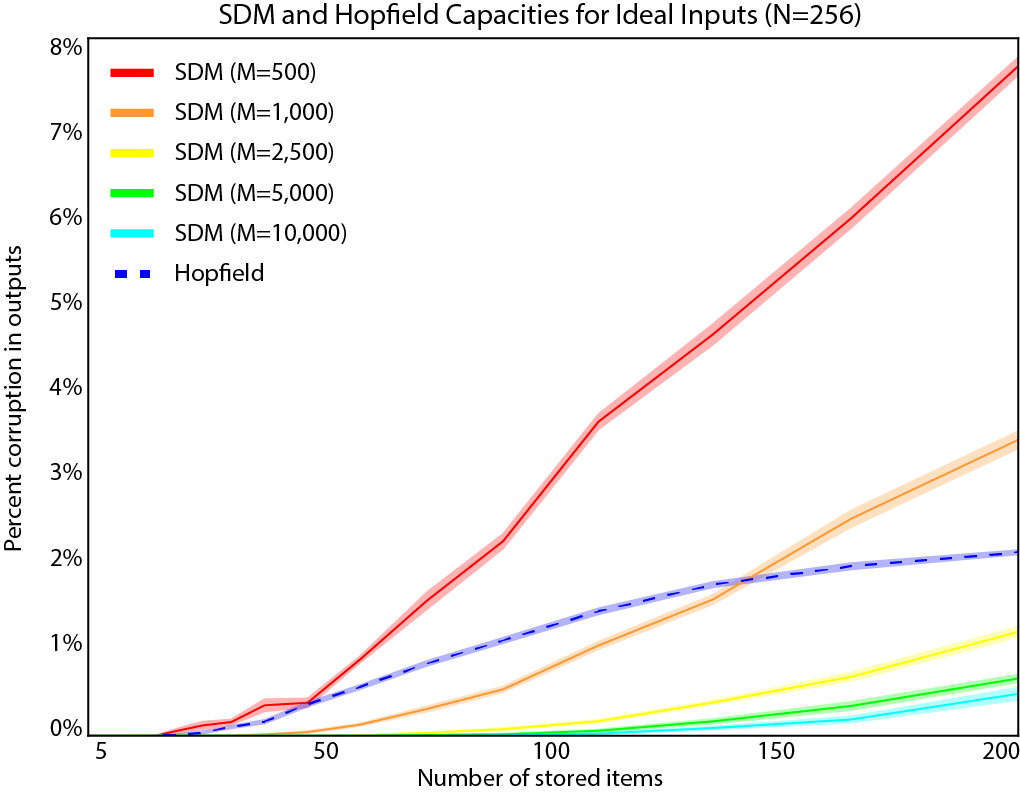
\includegraphics[width=0.8\textwidth]{./figures/capacity-edit.png}

\end{center}
\caption{This is a figure.} 
\label{sample-figure}
\end{figure}


\begin{figure}[ht!]
\begin{center}
	
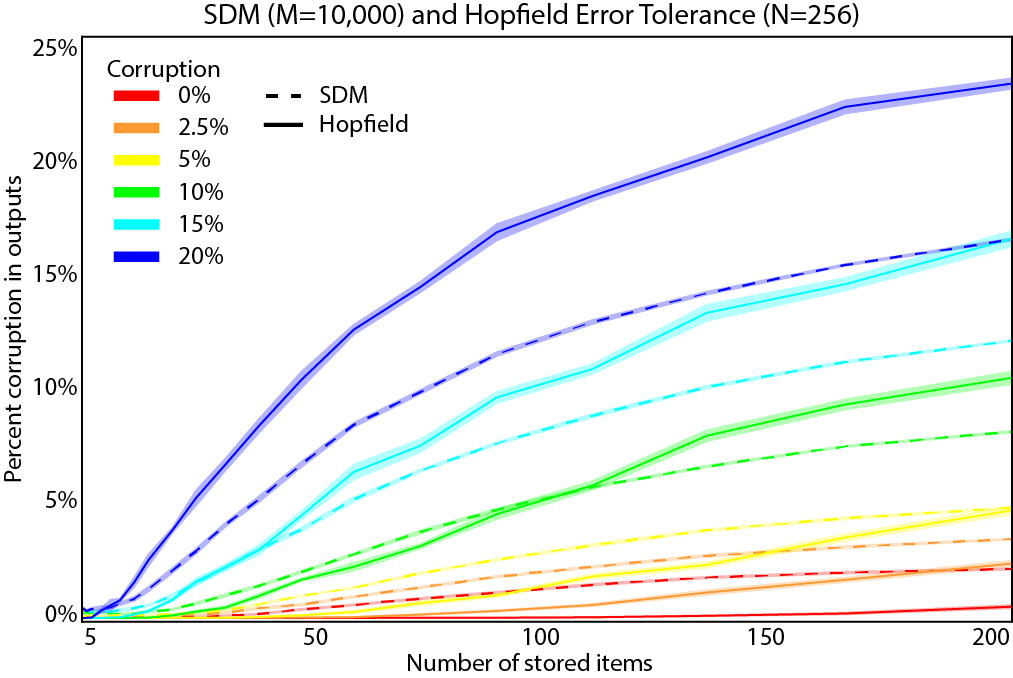
\includegraphics[width=0.8\textwidth]{./figures/tolerance-edit.png}

\end{center}
\caption{This is a figure.} 
\label{sample-figure}
\end{figure}

%%%%%%%%%%%%%%%%%%%%%%%%%%%%%%%%
% subsection - prototypes
%%%%%%%%%%%%%%%%%%%%%%%%%%%%%%%%
\subsection{Prototype Retrieval}

% what happens when we try to store the noisy circles in an hopnet, does it converge to a prototype as well?

% - even if it does, it can't really store much else without really messing things up due to its capacity, where in SDM it's just a tiny fraction of the space of things - ie, does storing noisy faces, numbers, circles, AND sequences do anything to the retrieval of the prototype?

\begin{figure}[ht!]
\begin{center}
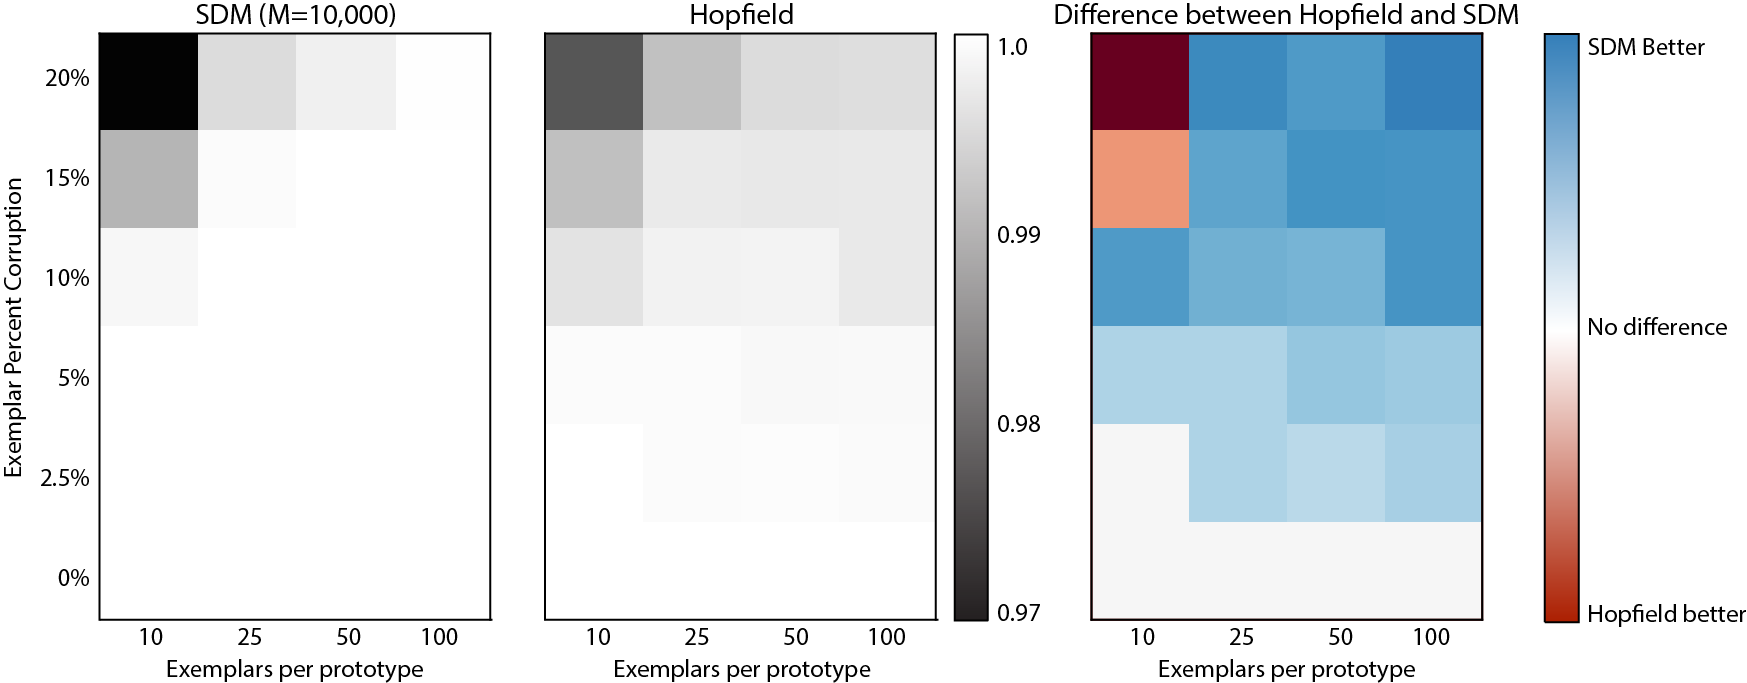
\includegraphics[width=0.95\textwidth]{./figures/prototype-edit.png}

\end{center}
\caption{This is a figure.} 
\label{sample-figure}
\end{figure}


%%%%%%%%%%%%%%%%%%%%%%%%%%%%%
% subsection - sequences
%%%%%%%%%%%%%%%%%%%%%%%%%%%%%
\subsection{Sequence Storage}

% just to show off here since the hopnet can't at all - but maybe we should make a comment about recurrent nets (JUST a comment) ?


%%%%%%%%%%%%%%%%%%%%%%%%%
% subsection - discussion
%%%%%%%%%%%%%%%%%%%%%%%%%
\subsection{Discussion}

% wrap up results from evaluations

% ** SDM is the best \\
% only the only model that is both robust to noise/storage capacity and
% sophisticated enough to behave in various ways 

** difference between addresses and data \\
% - address/data difference is called heteroassociative memory (associate one pattern with another - i think...)



%%%%%%%%%%%%%%%%%%%%%%%%%%%%%%%%%%%%%%%%%%%%%%%%%%%%%%%%%%%%%%%%%%%%%%
% future directions
%%%%%%%%%%%%%%%%%%%%%%%%%%%%%%%%%%%%%%%%%%%%%%%%%%%%%%%%%%%%%%%%%%%%%%
\section{Probabilistic interpretations of SDMs}

*** probabilistic interpretations \cite{Anderson1989}\\
*** figure out the encoding for importance sampling \\
*** how close does it have to be to the delta function? \\



%%%%%%%%%%%%%%%%%%%%%%%%%%%%%%%%%%%%%%%%%%%%%%%%%%%%%%%%%%%%%%%%%%%%%%
%  conclusions
%%%%%%%%%%%%%%%%%%%%%%%%%%%%%%%%%%%%%%%%%%%%%%%%%%%%%%%%%%%%%%%%%%%%%%
\section{Conclusions}



% \begin{table}[!ht]
% \begin{center} 
% \caption{Sample table title.} 
% \label{sample-table} 
% \vskip 0.12in
% \begin{tabular}{ll} 
% \hline
% Error type    &  Example \\
% \hline
% Take smaller        &   63 - 44 = 21 \\
% Always borrow~~~~   &   96 - 42 = 34 \\
% 0 - N = N           &   70 - 47 = 37 \\
% 0 - N = 0           &   70 - 47 = 30 \\
% \hline
% \end{tabular} 
% \end{center} 
% \end{table}

% \begin{figure}[ht]
% \begin{center}
% \fbox{CoGNiTiVe ScIeNcE}
% \end{center}
% \caption{This is a figure.} 
% \label{sample-figure}
% \end{figure}




%%%%%%%%%%%%%%%%%%%%%%%%%%%%%%%%%%%%%%%%%%%%%%%%%%%%%%%%%%%%%%%%%%%%%%
% bibliography
%%%%%%%%%%%%%%%%%%%%%%%%%%%%%%%%%%%%%%%%%%%%%%%%%%%%%%%%%%%%%%%%%%%%%%
\newpage
\bibliographystyle{apacite}

\setlength{\bibleftmargin}{.125in}
\setlength{\bibindent}{-\bibleftmargin}

\bibliography{classProject}


%%%%%%%%%%%%%%%%%%%%%%%%%%%%%%%%%%%%%%%%%%%%%%%%%%%%%%%%%%%%%%%%%%%%%%
% appendix (code)
%%%%%%%%%%%%%%%%%%%%%%%%%%%%%%%%%%%%%%%%%%%%%%%%%%%%%%%%%%%%%%%%%%%%%%
\newpage
\appendix

\section{Project Code}
This is where we have the code.


\end{document}
